% ===== DOUBLE-BLIND SUBMISSION build (Web3D 2026). =====
% For the CAMERA-READY, drop 'anonymous' below and re-enable \shortauthors.
\documentclass[sigconf,nonacm,screen,anonymous]{acmart}
\settopmatter{printacmref=false}
\usepackage{tikz}
\usetikzlibrary{positioning,arrows.meta}
\usepackage{booktabs}
\usepackage{balance}

\begin{document}

\title{Technē: A Deterministic Craft Layer for Model Context Protocol Servers, Grounded in LLM-Authored X3D}

\author{Alexander Hoffman}
\affiliation{%
  \institution{Independent Researcher}
  \country{USA}}
\email{alex@euphe.me}

% \renewcommand{\shortauthors}{Hoffman}   % LEAKS author in page headers under anonymous; re-enable for camera-ready

\begin{abstract}
A Model Context Protocol (MCP) server advertises its tools through a JSON Schema, so a language model can drive them by emitting typed tool calls. The schema is decidable and closed, yet it is the wrong success criterion: a model can emit calls that pass the schema in full and still produce a scene that renders mis-lit, mis-animated, or entirely blank. We name this the gap between epistēmē, the necessary formal structure a schema encodes, and technē, the contingent craft of making the artifact come out right that it does not. We present Technē, a deterministic craft layer that closes the gap for LLM-authored X3D over the Web3D x3d\_mcp server. Technē is a man-in-the-middle MCP proxy and makes three contributions. First, it redirects Schema-Aligned-Parsing-style repair plus craft validation onto the tool-call arguments a model emits into a server, intercepted in transport — inverting the app-to-model seam that productised tools occupy. Second, it compiles a written catalogue of X3D silent-failure modes into named, prescriptive corrections where the error message is the fix, so the craft holds mechanically whether or not the model comprehended it. Third, its occupation gate executes a renderer and inspects the pixels — verify-by-render — graduated by irreversibility, something no assertion language can do. Beyond X3D correctness, the same move extends to honesty: an opt-in provenance gate compiles the documented/interpretive/generated convention into deterministic checks against an asset ledger, so a feature cannot be labelled documented without the source that documents it. The system is built on BAML, carries 105 passing unit tests, is measured against the bare server in a controlled comparison, and is verified live end-to-end against the production server.
\end{abstract}

\ccsdesc[500]{Computing methodologies~Intelligent agents}
\ccsdesc[500]{Software and its engineering~Software verification and validation}
\ccsdesc[300]{Computing methodologies~Computer graphics}
\ccsdesc[300]{Information systems~Web services}
\ccsdesc[300]{Human-centered computing~Human computer interaction (HCI)}
\keywords{Model Context Protocol, LLM tool use, agentic systems, Schema-Aligned Parsing, BAML, X3D, HAnim, Web3D, deterministic validation, prescriptive correction, render-based verification, verify-by-render, occupation gate, craft, epistēmē, technē, man-in-the-middle proxy, data provenance, documented vs interpretive}

\maketitle


\begin{figure}[t]\centering
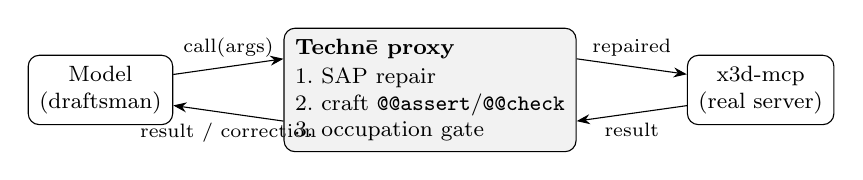
\begin{tikzpicture}[font=\footnotesize, >=Stealth, node distance=10mm,
  box/.style={draw, rounded corners, align=center, inner sep=4pt, minimum height=8mm}]
  \node[box] (model) {Model\\(draftsman)};
  \node[box, right=14mm of model, fill=black!5, align=left] (techne)
    {\textbf{Techn\=e proxy}\\[1pt]
     1.\ SAP repair\\
     2.\ craft \texttt{@@assert}/\texttt{@@check}\\
     3.\ occupation gate};
  \node[box, right=14mm of techne] (mcp) {x3d-mcp\\(real server)};
  \draw[->] (model.12) -- node[above,font=\scriptsize]{call(args)} (techne.168);
  \draw[->] (techne.12) -- node[above,font=\scriptsize]{repaired} (mcp.168);
  \draw[<-] (model.348) -- node[below,font=\scriptsize]{result / correction} (techne.192);
  \draw[<-] (techne.348) -- node[below,font=\scriptsize]{result} (mcp.192);
\end{tikzpicture}
\caption{Techn\=e as an MCP man-in-the-middle. Each \texttt{tools/call} is
repaired (Postel-style), validated against the craft rules, and either forwarded
with rewritten arguments or blocked with a prescriptive correction; the
occupation gate renders and inspects the result. Opt-in per tool.}
\label{fig:arch}
\end{figure}

\section{Introduction}\label{sec:intro}

The Model Context Protocol (MCP) gives a language model reach into external systems: a server advertises a set of named tools with JSON-Schema-typed arguments, and the model drives them by emitting structured tool calls~\cite{mcp,jsonschema}. The contract a tool advertises, however, is purely structural. A schema constrains the \emph{shape} of a call --- field names, value types, enumerations --- and a conforming validator will certify any call that fits. What it cannot certify is whether the operation the call requests is \emph{conventionally correct}: whether the edit it makes to a domain artifact will produce the thing the author intended. The protocol gives the agent reach; it does not give it craft.

The consequence is a failure mode that is easy to miss precisely because every checkable thing checks out. In our grounding domain --- X3D~4.0 scenes authored through the Web3D \texttt{x3d\_mcp} server~\cite{x3d4,x3dpy} --- a model can emit a sequence of tool calls that passes the X3D XSD in full and yet renders wrong, mis-lit, mis-animated, or entirely blank. A dropped \texttt{containerField} routes a humanoid's skeleton into the wrong parent slot and the figure renders invisible; a texture lands in a slot a physically based material does not define and a textured surface comes out flat. The validator reports success; the pixels report failure; nothing in between throws. The output is structurally valid but semantically dead.

We frame this as the gap between two kinds of knowledge that the philosophy of craft keeps distinct, and that a schema collapses. \emph{Epistēmē} is the necessary, decidable, closed formal structure --- the XSD and its object model, complete on its own terms and silent about everything it does not encode. \emph{Technē} is the contingent craft of making the thing come out right: which \texttt{containerField} routes which node into which parent slot, which defaults must be stated rather than assumed, which lengths must agree, which order operations must occur in. A digital-content-creation application supplies that technē implicitly, through enforced verbs and a fixed order of operations. X3D-the-format carries only epistēmē and assumes the technē lives in the authoring tool. When the author is a language model emitting raw tool-call arguments, that assumption fails, and the craft has nowhere to live.

This paper gives it somewhere to live. We present \emph{Technē}, a deterministic craft layer that sits as a man-in-the-middle on the MCP transport (Fig.~\ref{fig:arch}): the model connects to Technē, Technē launches the real server as a subprocess, and every tool call passes through a decision layer that repairs, validates, and --- at completion --- renders before the upstream server ever runs it. Built on BAML, the system makes three contributions, plus a fourth that extends the same discipline to provenance:

\begin{itemize}
  \item \textbf{In-transport redirection.} We point Schema-Aligned-Parsing-style argument repair and craft validation at the tool-call arguments a model emits \emph{into} an MCP server, intercepted in transit. Productised SAP applies this where application code calls a model (app$\rightarrow$model); Technē inverts the seam and applies it where a model calls a tool (model$\rightarrow$tool). No prior work points this discipline at tool-call arguments mid-flight in an MCP proxy.
  \item \textbf{Documented craft as mechanism.} We compile a written catalogue of X3D silent-failure modes --- output that passes the XSD yet renders wrong or blank --- into deterministic, named corrections where the error message \emph{is} the fix. The diagnostic a violation produces is a \emph{prescriptive correction} (``use \texttt{containerField=\textquotesingle{}baseTexture\textquotesingle{}}'') rather than a bare ``invalid,'' and the craft holds mechanically whether or not the model comprehended it.
  \item \textbf{The occupation gate.} We add an occupation gate that executes a renderer and inspects the pixels --- \emph{verify-by-render} --- something a schema validator or an assertion language, which only predicate over an already-parsed value, cannot do. The gate is graduated by irreversibility: a soft, automatic ``looks non-blank?'' check before cheap reversible work, and a hard human sign-off before expensive irreversible offline rendering.
  \item \textbf{The provenance bridge (a scope extension).} Beyond X3D correctness, the same documented-craft-into-mechanism move applies to honesty: an opt-in gate compiles the \emph{documented}/\emph{interpretive}/\emph{generated} provenance convention into deterministic checks against an asset ledger, so a feature cannot be labelled \emph{documented} without the source that documents it, and \emph{generated} geometry must disclose how it was made.
\end{itemize}

The remainder of the paper proceeds as follows. Section~\ref{sec:related} positions Technē against MCP tool use, the closed X3D and HAnim standards, Schema-Aligned Parsing and BAML, and prior LLM-driven Web3D authoring. Section~\ref{sec:gap} develops the epistēmē/technē gap through a catalogue of four documented X3D silent-failure modes. Section~\ref{sec:arch} presents the man-in-the-middle architecture and its governing commitment to determinism. Sections~\ref{sec:point2} and~\ref{sec:point3} detail the two built mechanisms: in-transport argument repair with prescriptive correction, and the occupation gate. Section~\ref{sec:eval} reports the implementation, 105 passing unit tests, a controlled comparison against the bare server, and a live end-to-end smoke verification against the production server. Section~\ref{sec:discussion} extends the discipline to a provenance bridge and discusses generalization beyond X3D and limitations, and Section~\ref{sec:conclusion} concludes.


\begin{figure}[t]\centering

\includegraphics[width=\columnwidth]{../figures/x3dom_vs_xite.png}
\caption{The renderer is a correctness property, not an aesthetic one. The same
scene under headless software WebGL: X3DOM (left) draws nothing for HAnim and X3D
4.0 \texttt{PhysicalMaterial}; \mbox{X\_ITE} (right) renders both. An X3DOM-based
occupation gate would inspect a blank and pass it.}
\label{fig:renderer}
\end{figure}

\section{Background and related work}\label{sec:related}

Technē sits at the confluence of four established lines of work: agentic tool use over the Model Context Protocol, the closed declarative standards of X3D and HAnim, deterministic schema-aligned parsing, and the small but growing literature on LLM-authored Web3D. We position the system against each, then state precisely what is new.

\subsection{MCP and LLM tool use}
The Model Context Protocol standardises how an agent discovers and invokes external \emph{tools}: a server advertises named operations with JSON-Schema-typed arguments, and the model drives them by emitting structured tool calls~\cite{mcp}. In our grounding domain the \texttt{x3d\_mcp} server exposes an editing surface over an X3D scene --- \texttt{create\_node}, \texttt{set\_field}, \texttt{add\_child}, \texttt{add\_route} --- so the agent operates a scene-graph editor rather than emitting a document in one shot~\cite{x3dpy}, and every mutation passes through a typed call on the wire, tractable to intercept. But a JSON-Schema argument type~\cite{jsonschema} constrains only the \emph{shape} of a call --- field names, value types, enumerations --- not whether the resulting edit is conventionally correct: the protocol gives reach, not craft.

\subsection{X3D 4.0 and HAnim as closed declarative standards}
X3D 4.0 is an ISO declarative scene-graph standard with a formally specified, closed schema---an XSD and an accompanying object model~\cite{x3d4,x3duom}. Its 4.0 revision adds the feature surface most exposed to silent failure: \texttt{PhysicalMaterial} physically based rendering aligned with glTF~\cite{gltf}, \texttt{EnvironmentLight} image-based lighting, and the articulated humanoids of the HAnim standard---\texttt{HAnimJoint}, \texttt{HAnimSegment}, and skinned coordinates~\cite{hanim}. Animation rides on interpolator nodes driven through \texttt{ROUTE}s, and node sharing rides on \texttt{DEF}/\texttt{USE}. The schema is \emph{epistēmē} in the sense developed in Sec.~\ref{sec:gap}: decidable, closed, silent about what it does not encode. Crucially, the same node type legally appears in several parent fields, distinguished only by \texttt{containerField}---a \texttt{HAnimJoint} as a \texttt{skeleton} root versus an ordinary \texttt{children} member; an \texttt{ImageTexture} as \texttt{baseTexture} versus the default \texttt{texture} slot. Which \texttt{containerField} belongs in which slot is contingent craft knowledge the XSD does not express, and getting it wrong yields output that validates yet renders blank --- the class the \texttt{x3d.py} bug report documents~\cite{x3dpy}. Conformant players (\texttt{X\_ITE}~\cite{xite}, \texttt{X3DOM}~\cite{x3dom}, Castle Model Viewer~\cite{castle}) faithfully render the wrong thing, because the document is, by the schema's lights, correct; the canonical X3D Examples Archive embodies this craft by convention, not enforcement~\cite{x3dexamples}.

\subsection{Schema-Aligned Parsing and BAML}
BAML productises Schema-Aligned Parsing (SAP): deterministic, edit-distance repair of a model's loosely structured output into a target schema, following Postel-style liberal acceptance~\cite{baml,postel}, paired with validation as first-class constructs --- \texttt{@@assert} (blocking) and \texttt{@@check} (advisory) --- that let craft predicates live in the schema rather than in scattered procedural checks. Technē builds \emph{on} BAML, adopting both its repair engine and its assertion semantics; the decisive difference is topology. BAML sits where application code calls a model (the \emph{app$\rightarrow$model} seam); the MCP problem is the inverse --- a model calls a tool, and the arguments needing repair are the ones it emits \emph{into} the server, intercepted in-transport (Fig.~\ref{fig:arch}). No prior work points SAP-style repair and craft validation at tool-call arguments mid-flight in an MCP proxy. We inherit BAML's constraints honestly: only block-level \texttt{@@} assertions fire at runtime, and a raised error blurs \emph{which} assertion failed --- so every rule is named and mapped to a prescriptive correction, preserving the identity the catalogue depends on.

\subsection{LLM-driven X3D authoring and AI for Web3D}
Prompt engineering for LLM-authored X3D has been studied directly: careful prompts measurably improve the rate at which a model emits usable scenes~\cite{prompteng}. That work operates on the \emph{advisory} side of the determinism boundary---it shapes what the model probably does, and the gains reset when a fresh model connects. Adjacent AI-for-Web3D work pursues accessibility and quality, such as automated audio captioning of scenes~\cite{audiocaption}. Technē is complementary and orthogonal: rather than improving the prompt, it makes the craft hold mechanically downstream of whatever the model emitted, so comprehension is no longer load-bearing.

\subsection{Blackboard architectures and guardrails}
The blackboard architecture is a useful prior frame for staged cooperation among heterogeneous agents writing to a shared evolving solution under a control regime~\cite{blackboard}; Technē's human-architect / model-draftsman / deterministic-discipline split is a narrow, modern instance, with the scene as the shared structure and the gate as the control. More broadly, validation and guardrail layers and JSON-Schema tool contracts~\cite{jsonschema} predicate over an \emph{already-parsed value}: they answer ``is this argument well-formed?'' They cannot answer ``did the moose render as a moose,'' because that is side-effecting computation outside assertion scope.

\subsection{What is new in Technē}
Against this background, the contributions enumerated in Sec.~\ref{sec:intro} are original: the in-transport redirection of SAP-style repair onto tool-call arguments (a man-in-the-middle inversion of BAML's app$\rightarrow$model seam~\cite{baml,mcp}), documented-craft-as-mechanism~\cite{x3dpy}, the occupation gate, and the provenance bridge --- none of which prior LLM-for-Web3D work~\cite{prompteng} provides. The renderer choice is itself a correctness property: X3DOM draws blank headless what X\_ITE renders fully (Fig.~\ref{fig:renderer}; see Sec.~\ref{sec:point3}).

\section{The craft gap: structurally valid, semantically dead}\label{sec:gap}

An MCP server~\cite{mcp} exposes a domain as a flat surface of tools and node types; for X3D~\cite{x3d4} authored through the Web3D \texttt{x3d\_mcp} server every verb maps to a legal operation and every document checks against the X3D~4.0 XSD via the X3D Unified Object Model~\cite{x3duom}. As Sec.~\ref{sec:intro} framed it, schema conformance is nonetheless the wrong success criterion: a model emitting tool calls into this surface can produce a document that passes the XSD in full yet renders wrong, mis-lit, mis-animated, or blank --- the validator reports success, the pixels report failure, and nothing in between throws. This is the gap between \emph{epistēmē}, the decidable closed structure the XSD encodes, and \emph{technē}, the contingent craft it does not: which \texttt{containerField} routes a node into which parent slot, which defaults must be stated rather than assumed, which lengths must agree, which order operations must occur in. A digital-content-creation application supplies that craft implicitly through enforced verbs and a fixed order of operations; X3D-the-format carries only epistēmē and assumes the technē lives in the authoring tool, so when the author is a language model emitting raw arguments the craft has nowhere to live.

The concrete content of this gap is a small, documented catalogue of \emph{silent-failure modes}: outputs that pass the schema yet break rendering. We draw four from the \texttt{x3d.py} bug report (\texttt{docs/x3dpy-bug-report.md})~\cite{x3dpy} while building HAnim humanoids and PBR scenes programmatically, serializing with \texttt{X3D(...).XML()}, and rendering in a conformant viewer. They share one signature, developed below: none throw, all validate, all fail only when a renderer runs and a human looks.

\subsection{Dropped \texttt{containerField}}
Every X3D node has a default \texttt{containerField} --- the slot it lands in when none is stated (\texttt{HAnimJoint}$\to$\texttt{children}, \texttt{ImageTexture}$\to$\texttt{texture}). But many nodes legally appear in more than one parent field, and a node placed in a non-default slot must name it explicitly or a conformant reader files the child into its default field instead. \texttt{x3d.py} serializes such a node with no \texttt{containerField} at all: a skeleton root supplied through \texttt{HAnimHumanoid.skeleton} emits without \texttt{containerField='skeleton'}, so the player routes it into \texttt{children} and the entire humanoid~\cite{hanim} renders invisible. The same defect drops PBR textures --- an \texttt{ImageTexture} meant for \texttt{baseTexture} of a \texttt{PhysicalMaterial}~\cite{gltf} keeps its default \texttt{texture} slot, which the material does not define, so a textured surface renders as flat base color. Technē's catalogue enumerates the legal slots per material and per humanoid, so a missing or wrong container is rejected with the exact slot to use.

\subsection{\texttt{EnvironmentLight.global}}
The X3D~4.0 Lighting table specifies \texttt{SFBool global FALSE} for \texttt{EnvironmentLight}; \texttt{x3d.py} defaults it to \texttt{True} (matching the point and spot lights) and --- because serializers omit fields equal to their internal default --- drops \texttt{global} from the output even when the author set it true. A spec-default reader parses the absent attribute as \texttt{false}, so the light is not global and image-based ambient lighting silently dies, the scene lit only by whatever direct lights remain. The divergence cannot be repaired in the tool arguments because that default never reaches the wire; the correction must inject \texttt{global='true'} at the serialization layer.

\subsection{Interpolator \texttt{key}/\texttt{keyValue} length mismatch}
An interpolator's \texttt{keyValue} array must hold exactly \texttt{len(key)} entries times the node's per-key component count --- four for \texttt{OrientationInterpolator}, three for \texttt{PositionInterpolator}, one for \texttt{ScalarInterpolator}. The XSD types both fields as float arrays and checks neither their relative length nor the multiple. A mismatch passes validation and silently corrupts the animation, shifting or truncating keyframes with no error.

\subsection{USE-before-DEF ordering}
A \texttt{USE} reference must follow the \texttt{DEF} it names. Emit the \texttt{USE} first and the document is still well-formed XML and schema-valid, but the reference resolves to nothing and the reused geometry vanishes. This is an order-of-operations constraint --- pure technē --- that no per-element schema check can see.

The four modes share their defining property: each produces output that \emph{passes XSD schema validation} yet renders incorrectly, because the defect lives in container routing, a non-spec default, a cross-field length relation, or an ordering constraint --- none of which the schema predicates over. This is precisely the craft a DCC application supplies through enforced verbs and order of operations, and which X3D-the-format leaves to live elsewhere. The remainder of this paper is about giving it somewhere to live: a deterministic layer that holds the technē mechanically, in transport, whether or not the model comprehended it.

\section{Technē: architecture}
\label{sec:arch}

Technē is a man-in-the-middle for the Model Context Protocol~\cite{mcp}. The model connects not to the x3d-mcp server but to Technē, which launches the real server as a subprocess and connects to it as a client (Fig.~\ref{fig:arch}); every \texttt{tools/call} passes through a decision layer before the upstream ever runs it, and every result passes back through before the model sees it. To the model the surface is unchanged --- the same tool names and arguments --- save a one-line hint on guarded tools that their arguments are repaired and validated in transit. This transport position is the load-bearing choice: BAML~\cite{baml} applies Schema-Aligned Parsing where \emph{code calls a model} (app$\rightarrow$model), and Technē inverts the seam onto the arguments \emph{a model emits into a tool} (model$\rightarrow$tool). Nothing in the decision logic depends on the wire format, so the same core would front any MCP server; X3D via \texttt{x3d\_mcp}~\cite{x3dpy} is the grounding domain, not a dependency.

\subsection{The governing commitment: determinism}

The design answers a single failure of advice. Craft-rules written into a server's prose \texttt{instructions} --- ``set \texttt{containerField} explicitly off the default slot'' --- are advisory: the model \emph{probably} reads and applies them, and the dice reset the moment a fresh session connects. Technē instead makes the craft hold \emph{mechanically}: the arguments pass \emph{through} a layer that repairs and validates them deterministically before the real server runs them, so a correction discovered once becomes mechanism the next model cannot ignore rather than text it must re-comprehend --- Postel-style liberal acceptance~\cite{postel} relocated to transform what the model emits before it acts. The corollary, deliberate: the runtime path performs no per-call LLM round-trip --- the validation is a deterministic Python mirror of the canonical BAML declarations in \texttt{baml\_src/}, so a layer whose whole claim is determinism does not reintroduce a model into its own enforcement.

\subsection{The per-call pipeline}

For each call, \texttt{decide()} (in \texttt{proxy.py}) runs three steps. \emph{First}, deterministic SAP-style repair (\texttt{repair.py}) coerces the raw arguments into conforming shape --- the proxy sets \texttt{validate\_input=False} precisely so Technē sees the model's raw, possibly sloppy arguments before any upstream schema check can reject them. \emph{Second}, routing: a tool with a registered craft adapter runs through it, one without forwards unchanged --- an opt-in stance that is a claim about the catalogue (no rule means no documented failure mode there), not an omission. \emph{Third}, the decision: the adapter returns a \texttt{CraftResult} that either rewrites-and-forwards a repairable argument set or \emph{blocks} the call --- the call never reaches the real server --- and returns the prescriptive correction in its place, the error message standing in as the fix (``Use \texttt{containerField=\textquotesingle{}skeleton\textquotesingle{}}''), not a bare ``invalid'' (Sec.~\ref{sec:point2}). The asymmetry is the point: a violation whose correct value is determinable is repaired silently and forwarded; one that is not is blocked and handed back to the architect's draftsman to redo.

This is Point 2 of the specification --- in-call argument repair plus structural validation --- and it is built. It is sequence-agnostic: it inspects one call's arguments (in concert with minimal scene memory, below) and needs no model of the whole authoring session.

\subsection{Minimal scene state}

Some craft-rules are structural but not local: checking a child's \texttt{containerField} against its parent needs the \emph{types} of both, yet \texttt{add\_child} references nodes by opaque \emph{id}. Technē therefore keeps a minimal \texttt{SceneState} --- an \texttt{id}$\rightarrow$type map, the \texttt{DEF} names seen, and the field values set --- committed only on confirmed upstream success through the deferred \texttt{decide()}/\texttt{observe\_result()} split detailed in Sec.~\ref{sec:point2}: a ledger of confirmed facts about the scene, never of attempts.

\subsection{The occupation gate}

Point 3, also built, is the occupation gate (Sec.~\ref{sec:point3}). Repair and validation predicate over arguments; the gate \emph{executes a renderer and inspects the pixels} --- something no schema validator~\cite{jsonschema} and no assertion language can do, since both reason only over an already-parsed value (Sec.~\ref{sec:point3}). The gate is graduated by irreversibility (Fig.~\ref{fig:gate}): a cheap, soft, automatic ``looks non-blank?'' check fires on render verbs and appends a warning when the returned image carries no visible geometry, while a hard human sign-off guards the expensive, irreversible offline render. Its teeth depend on the renderer that can actually draw the scene: X3DOM~\cite{x3dom} draws blank headless what X\_ITE~\cite{xite} renders fully for an HAnim~\cite{hanim} humanoid (Fig.~\ref{fig:renderer}; see Sec.~\ref{sec:point3}), so the backend is itself a correctness property.

\subsection{What is deliberately not built}

Point 1 --- a cross-call automaton enforcing order-of-operations over the whole session --- is intentionally absent. Open-ended authoring should resist a straitjacket: which scene to build, and where, is the human architect's free field, not a defect to regiment. The likely truth is a partial order, a few hard edges in a large open space, so Technē instruments first (logging the verb order of clean renders) and lets usage vote before any automaton is committed. The framing throughout is the draftsman's: the human architect holds intent and signs off; the model is the fast draftsman who knows the conventions but does not originate intent; Technē is the draftsman's discipline plus the commitment gate --- it makes the draft conform and holds the boundary before irreversible work, and reaches into neither the intent nor the sign-off.

\section{Repairing and validating tool-call arguments}\label{sec:point2}

Point~2 is the layer that sits between the model's emitted \texttt{tools/call} and the real x3d-mcp server~\cite{mcp}, and decides, per call, whether the arguments may be forwarded as written, rewritten and forwarded, or refused with a correction (Figure~\ref{fig:arch}). It runs in two stages: a deterministic \emph{repair} of argument shape (\texttt{repair.py}), followed by a catalogue of \emph{craft} rules over the cleaned arguments (\texttt{craft.py}, \texttt{rules.py}). Both stages are LLM-free Python, honouring the determinism commitment (Sec.~\ref{sec:arch}); the canonical BAML declaration in \texttt{baml\_src/craft.baml} mirrors them and is the path to BAML's Schema-Aligned Parsing (SAP) when wired.

\subsection{SAP-style argument repair}
The first stage applies Postel's robustness principle---``be liberal in what you accept''~\cite{postel}---to the tool-call arguments, the move BAML productises as SAP for model \emph{output}~\cite{baml}, here redirected onto the arguments a model emits \emph{into} a tool. \texttt{sap\_repair} is deliberately conservative: it unwraps and coerces shape but never invents content. It strips markdown fences and any chain-of-thought preceding the first JSON object; un-stringifies values under structured keys (\texttt{fields}, \texttt{value}, \texttt{arguments}, \texttt{args}) that arrived as embedded JSON text; and coerces obvious scalar leaves---\texttt{"true"}/\texttt{"false"} to bool, numeric strings to numbers---only where a boolean or numeric field is expected (e.g.\ a \texttt{global} leaf inside \texttt{fields}). It never raises: worst case it returns the original dict or \texttt{\{\}}, so the caller can still forward. This is the conformance-shaping layer; the semantic rules run only on the result. When the generated BAML client is present, \texttt{b.parse.<Function>(json)} substitutes the full edit-distance engine for this dependency-free baseline.

\subsection{The rule-to-fix catalogue}
The second stage is the documented craft. We reread the catalogue of X3D silent-failure modes---constructs that pass the XSD yet render wrong or blank---as a table \texttt{\{rule: (severity, prescriptive-correction, source)\}} in \texttt{rules.py}. Each entry names a single assertion and maps it to a \emph{prescriptive} correction string, not a bare ``invalid.'' The whole point is the difference between ``rejected'' and ``rejected: use \texttt{containerField='baseTexture'}''. A thrown XSD or assertion error reports only that \emph{some} predicate over the parsed value failed; it blurs which assertion it was and says nothing about the fix. By naming every rule (\texttt{container\_field\_present}, \texttt{container\_field\_correct}, \texttt{container\_field\_required}, \texttt{container\_field\_invalid\_slot}, \texttt{interp\_lengths\_match}, \texttt{use\_after\_def}, \texttt{envlight\_global\_set}, \ldots) and binding it to a templated correction carrying the offending node type, field, and the legal alternatives, the error message \emph{is} the fix. Each entry cites its source---most to the \texttt{x3d.py} bug report (\texttt{docs/x3dpy-bug-report.md})~\cite{x3dpy}, the rest to the Technē specification---so the craft is traceable, not folklore. Severity is binary: \texttt{HARD} rules block (mirrored as BAML \texttt{@@assert}); \texttt{SOFT} rules advise (\texttt{@@check}).

\subsection{Two outcomes: repair, or block-and-correct}
A craft rule resolves to one of two outcomes, and the discriminator is whether the correct value is \emph{determinable} without guessing intent. \emph{Repair} fires when exactly one legal value exists: a \texttt{containerField} must equal the field the node is placed in, and a placement with a single legal slot has one answer. Here Technē rewrites the argument, records a note, and forwards the corrected call, so the craft holds mechanically whether or not the model comprehended it. \emph{Block-and-correct} fires when the fix needs a choice the layer cannot make: which of \texttt{baseTexture}/\texttt{normalTexture}/\texttt{occlusionTexture} a texture was meant for; which \texttt{DEF} a dangling \texttt{USE} intended; or which of \texttt{key} and \texttt{keyValue} is the wrong length when their parity fails. In these cases Technē refuses to forward and returns the prescriptive correction listing the legal slots, leaving the intent decision to the model on retry. Filling it in would be inventing content---the very thing the repair stage forbids. The outcomes compose: \texttt{CraftResult} carries \texttt{repaired} arguments, a \texttt{corrections} list (any non-empty list blocks the forward), \texttt{notes}, and the \texttt{applied} rule names, and \texttt{merge} folds several single-rule results into one.

\subsection{A worked example: the texture containerField}
Consider a model that places an \texttt{ImageTexture} under a \texttt{PhysicalMaterial} via \texttt{add\_child} with no \texttt{containerField}. The XSD is satisfied --- \texttt{ImageTexture} is a legal child --- so a schema validator passes it, yet its default \texttt{texture} slot is one a PBR material~\cite{gltf} does not define, and the surface renders untextured. Technē looks up the two types in its scene state, finds \texttt{(PhysicalMaterial, ImageTexture)} in \texttt{MATERIAL\_TEXTURE\_SLOTS} with five legal slots, and --- because more than one is legal --- does not guess: it blocks and returns \texttt{container\_field\_required}, naming the child, the parent, the silently-dropped default, and the five slots. Had the parent been an \texttt{HAnimHumanoid}~\cite{hanim} with an \texttt{HAnimSegment} child, whose only non-default slot is \texttt{segments}, the same machinery would repair --- set \texttt{containerField='segments'} and forward --- because the answer is unique. One mechanism, two outcomes, decided by slot cardinality.

\subsection{The stateful proxy}
The containerField rule needs the child and parent \emph{types}, but \texttt{add\_child} references nodes by \emph{id}~\cite{x3duom}, learned only from \texttt{create\_node} responses, so \texttt{TechneProxy} keeps the minimal \texttt{SceneState} of Sec.~\ref{sec:arch} (\texttt{id\_to\_type}, \texttt{node\_fields}, \texttt{defined\_defs}, \texttt{def\_name\_to\_type}). Its correctness hinges on \emph{deferred commit}: \texttt{decide()} only reads state and records what it \emph{would} commit; \texttt{observe\_result()} commits the id$\rightarrow$type, \texttt{DEF}, and field updates only after a confirmed-successful upstream response --- so a failed \texttt{create\_node} registers no type, and a premature \texttt{DEF} from a failed \texttt{def\_node} cannot satisfy a later \texttt{USE}. When the proxy cannot resolve a type, it degrades to a non-blocking note rather than a false correction.

\subsection{The canonical BAML mirror}
\texttt{baml\_src/craft.baml} declares the same modes as block-level \texttt{@@assert}/\texttt{@@check} over classes (\texttt{TextureAttachment}, \texttt{EnvironmentLightArgs}, \texttt{InterpolatorArgs}, \texttt{UseRef}). It is the source of truth and the SAP path; the Python engine is its deterministic, runnable mirror. One trap is load-bearing: only the \emph{double}-\texttt{@} block form fires --- field-level single-\texttt{@} assertions are silently ignored at runtime, the very class of silent failure the layer exists to catch. The \texttt{EnvironmentLight.global} case marks the layer's boundary honestly: because that divergence lives below the wire (Sec.~\ref{sec:gap}), the args layer \emph{cannot} repair it, so Technē demotes it to a \texttt{SOFT} advisory here and pushes the hard fix into the serialization step at the gate (Figure~\ref{fig:gate}), which injects \texttt{global='true'} into the XML directly.

\subsection{Beyond create: edit verbs and standing semantics}
Two layers carry the same discipline past the create/\texttt{add\_child} surface. The content-edit verbs --- \texttt{modify\_x3d\_node}, \texttt{move\_x3d\_node}, \texttt{remove}, \texttt{convert} --- mutate an existing document and report success without re-checking it, so Technē \emph{post-validates} their results: an XSD post-pass catches a misspelled attribute a \texttt{modify} wrote, a semantic post-pass re-checks the \texttt{containerField} a \texttt{move} never revisited, and an element-count diff flags the nodes a \texttt{convert} silently dropped --- faults no single validator reports on its own. Separately, a standing-semantics layer (\texttt{semantics.py}) surfaces the invariants a session forgets --- X3D is right-handed and in metres and radians; a \texttt{TimeSensor} animates only through \texttt{ROUTE}s; an \texttt{HAnimJoint}'s rest pose is identity --- as soft reminders that ride back on the relevant tool result, deterministically, where a prompt read once at the top of a session would have lapsed.

\section{The occupation gate: render and look}\label{sec:point3}

The two preceding mechanisms operate on values: schema-aligned repair rewrites the arguments a model emits, and the craft rules predicate over an already-parsed scene to assert that the conventions the XSD does not encode are nonetheless satisfied. Both are, in the end, functions from a structure to a verdict. This is also the ceiling of an assertion language. A BAML \texttt{@@assert} or \texttt{@@check}~\cite{baml}, like a JSON Schema keyword~\cite{jsonschema} or an XSD facet, can only quantify over the parsed term in front of it; it cannot leave the term, \emph{execute a renderer}, get pixels back, and assert that those pixels are non-blank. Yet that is precisely the test the X3D silent-failure modes demand: a dropped \texttt{containerField} or a wrong \texttt{EnvironmentLight.global} produces a document that satisfies every predicate one can write over the document and still renders to an empty frame. The verdict that matters is not a property of the term but of its image. The occupation gate is the layer that crosses that boundary --- it executes a renderer and inspects the pixels, the principle we name \emph{verify-by-render} --- the genuinely original piece, the part for which there is no assertion-language analogue, because it is side-effecting by construction.

\subsection{The gate's logic}

The gate fires on a completion signal --- the moment a model declares the artifact done --- and runs three stages in dependency order (\texttt{techne/gate.py}). First, the semantic validator; if the output is not clean, it blocks and returns the validator's errors verbatim as corrections, so a structurally dead scene never reaches the renderer (``clean'' is read leniently --- an empty string or any of the upstream's all-clear markers --- to stay faithful to the real \texttt{validate\_semantic}). Second, it renders the scene and reduces the PNG to a single luminance figure --- the standard deviation across pixels --- treating anything below a small threshold (\texttt{BLANK\_STDDEV}, three grayscale levels) as blank: a flat, all-background frame with no geometry. This is the silent failure \emph{only} the render catches, so the correction is specific --- check that geometry is present, lit, on-camera, and that the HAnim and PBR \texttt{containerField}s are correct --- rather than a bare ``invalid.'' Third, only once the frame is non-blank, the gate applies a sign-off proportional to what is downstream.

A design commitment runs through the blank check: \emph{fail safe}. The inspector decodes the PNG with Pillow, or falls back to the IHDR dimensions and sampled scanlines when Pillow is absent; but if it cannot decode the image at all it returns \texttt{non\_blank = False} --- an image we cannot inspect is treated exactly as a blank one, and blocks. The asymmetry is deliberate: a false block costs a retry, a false pass ships a blank artifact, and the second failure is the one nothing else catches.

\subsection{The renderer is a correctness property}

The gate is only as honest as its eyes, so the choice of renderer stops being an implementation detail and becomes a correctness property (Fig.~\ref{fig:renderer}). Under headless software WebGL, X3DOM renders \emph{blank} for exactly the content this project showcases --- HAnim humanoids and X3D~4.0 \texttt{PhysicalMaterial} surfaces --- while X\_ITE renders both~\cite{xite,x3dom,gltf,playwright}. A gate wired to X3DOM would read a perfectly correct skeleton as a zero-variance blank and --- unable to tell an authoring error from the renderer's own incapacity --- block every valid figure, or, with the polarity flipped, certify blanks as fine. Its verdict would be a property of the renderer, not the scene. So the gate's hard prerequisite is X\_ITE: for an adjudicator that decides by looking, the renderer that can actually display the content is the only one that tells the truth.

\subsection{Graduation by irreversibility}

The sign-off is graduated by how irreversible the work it guards is (Fig.~\ref{fig:gate}); the frame is the architect and the draftsman (Sec.~\ref{sec:arch}), the human signing off, the model never pouring concrete on its own authority. A cheap, fast preview render is reversible, so the gate before it is soft and automatic, wired directly into the transport (\texttt{techne/server.py}): on the render verbs (\texttt{render\_image}, \texttt{render\_current\_scene}) the proxy inspects the returned image and, if blank, appends an occupation-gate warning to the relayed result --- in-band, on every render, at no extra round-trip. The expensive, hours-long offline photoreal render is the irreversible, pour-concrete moment, and the gate before it is \emph{hard}: when the cost is marked expensive and the human sign-off has not returned approval, the gate surfaces the validated preview and \emph{stops}, returning \texttt{awaiting\_architect}; its default sign-off returns false, so expensive work always waits by construction. This hard gate is host-driven --- the upstream exposes no offline-render verb to attach it to yet, so it lives in the \texttt{OccupationGate} library awaiting that verb, while the cheap gate already runs in transport. The discipline scales with the stakes --- a glance before reversible drafting, a human signature before irreversible building.

\begin{figure}[t]\centering
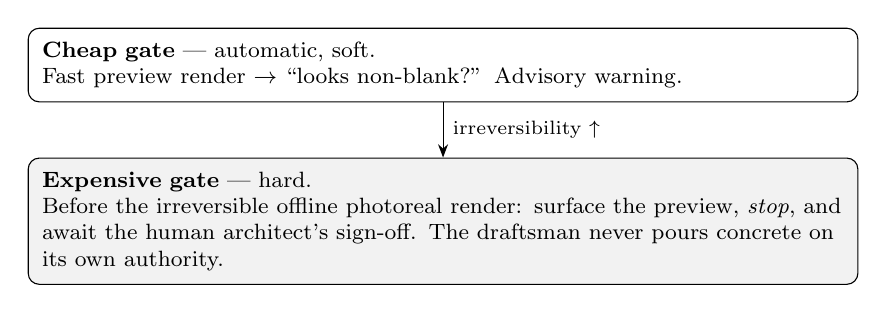
\begin{tikzpicture}[font=\footnotesize, >=Stealth,
  box/.style={draw, rounded corners, align=left, inner sep=5pt, text width=0.84\columnwidth}]
  \node[box] (cheap) {\textbf{Cheap gate} — automatic, soft.\\
     Fast preview render $\rightarrow$ ``looks non-blank?'' Advisory warning.};
  \node[box, below=7mm of cheap, fill=black!5] (exp)
    {\textbf{Expensive gate} — hard.\\
     Before the irreversible offline photoreal render: surface the preview,
     \emph{stop}, and await the human architect's sign-off. The draftsman never
     pours concrete on its own authority.};
  \draw[->] (cheap) -- node[right,font=\scriptsize]{irreversibility $\uparrow$} (exp);
\end{tikzpicture}
\caption{The occupation gate is graduated by irreversibility: a soft check before
cheap reversible work, a hard human sign-off before expensive irreversible work.}
\label{fig:gate}
\end{figure}

\section{Implementation and evaluation}\label{sec:eval}

Techn\=e is a small Python package that sits in front of the Web3D \texttt{x3d\_mcp} server~\cite{x3dpy} as a man-in-the-middle MCP proxy (Figure~\ref{fig:arch}). The implementation is deliberately modest in size and dependencies, because its claim is mechanistic rather than statistical: the craft must hold deterministically on every call, so the runtime that enforces it is the artifact under test.

\subsection{Implementation}

The package decomposes along the three insertion points of Section~\ref{sec:arch}. \texttt{rules.py} is the rule-to-fix catalogue --- the documented modes reread as a table mapping each rule name to a \emph{(severity, prescriptive correction, source)} triple, reconciled with the production server's own \texttt{validate\_semantic} so the layer names the same modes the whole-scene validator checks. \texttt{craft.py} implements the four modes of Sec.~\ref{sec:gap} through the repair / block-and-correct outcomes of Sec.~\ref{sec:point2}; \texttt{repair.py} is the dependency-free SAP-style argument repair mirroring BAML's \texttt{b.parse}~\cite{baml} --- unwrapping stringified field dicts, stripping markdown fences and preamble, coercing scalars in the spirit of Postel-style liberal acceptance~\cite{postel}. \texttt{proxy.py} is the stateful decision core, building scene state from \texttt{create\_node} results and splitting \texttt{decide()}/\texttt{observe\_result()} so state commits only on confirmed upstream success. \texttt{gate.py} is the occupation gate (Figure~\ref{fig:gate}), \texttt{server.py} the MCP transport, and \texttt{baml\_src/} the canonical BAML declaration of the same rules as block-level \texttt{@@assert}/\texttt{@@check}, each named back to the catalogue. \texttt{semantics.py} carries the standing invariants and \texttt{provenance.py} the opt-in provenance gate with its ledger checks; \texttt{config.py} holds the per-deployment profiles that switch extensions such as provenance on, and \texttt{eval/} is the scripted-and-live evaluation harness.

The runtime depends only on the \texttt{mcp} SDK for the stdio transport, Pillow for the gate's pixel inspection (its ``eyes''), and the Python standard library; the craft and repair engines are dependency-free so Techn\=e runs without a per-call LLM round-trip, faithful to the determinism commitment (Sec.~\ref{sec:arch}). Because \texttt{x3d\_mcp} is itself a Python MCP server, the proxy and the upstream can be co-located: \texttt{python -m techne.server -{}- python .../src/server.py} launches the real server as a subprocess and connects to it as a client, so the entire man-in-the-middle is one process tree. The model connects to Techn\=e; everything after \texttt{-{}-} is the upstream. \texttt{list\_tools} forwards the upstream surface, tagging Techn\=e-guarded tools in their descriptions; \texttt{call\_tool} runs the decision core, answering a hard violation with the prescriptive correction (the call never reaches the real server), forwarding repaired arguments otherwise, and appending the cheap blank-render warning on render verbs.

\subsection{Unit evaluation}

The package carries 105 unit tests. The craft tests exercise each documented mode in both directions: a missing or wrong \texttt{containerField} repaired to the correct slot while a correctly-placed node is left alone; a mismatched interpolator \texttt{key}/\texttt{keyValue} blocked with a correction naming the expected and actual lengths; a \texttt{USE} with no prior \texttt{DEF} blocked; a non-image texture URL warned without blocking. The proxy tests cover the stateful surface a stateless validator cannot: placement checked against the registered node type; the single-legal-slot case (an \texttt{HAnimSegment} under an \texttt{HAnimHumanoid}) repaired versus the multi-slot case (a texture under a \texttt{PhysicalMaterial}) that must block because the right answer cannot be guessed; \texttt{USE}-reference type inheritance, so a placed \texttt{USE} is still checked; and failed creates or \texttt{DEF}s that must \emph{not} register, so a later \texttt{USE} still blocks. The SAP-repair tests confirm the unwrapping and never-raises contract; the gate tests verify blank-versus-non-blank discrimination, the cheap/expensive graduation, and that the gate recognizes the \emph{actual} \texttt{validate\_semantic} string the real server emits, not a mock's; and the transport tests confirm guarded-tool tagging, that a blocked call never forwards while still returning its prescriptive correction, that the \texttt{EnvironmentLight} advisory is relayed without injecting a breaking argument, and that the blank-render warning is appended. Further suites cover the edit-verb post-pass (a misspelled \texttt{modify}, an un-rechecked \texttt{move}, a node-dropping \texttt{convert}), the standing-semantics reminders, and the provenance gate at L1--L2 --- an undisclosed \texttt{generated} asset, a \texttt{documented} claim with no ledger entry --- which stays silent until a profile opts in.

\subsection{Controlled comparison}

The layer's value is the difference between driving an authoring task through the bare server and through Techn\=e, so we measure it directly. A fixed set of six short authoring sequences runs through \texttt{x3d\_mcp} twice --- once raw, once behind Techn\=e, in isolated processes; five carry a documented silent-failure mode (a texture without its \texttt{containerField}; an interpolator whose \texttt{keyValue} length contradicts its \texttt{key} count; a \texttt{USE} before its \texttt{DEF}; a duplicate \texttt{DEF}; a \texttt{ROUTE} whose endpoints carry no \texttt{DEF}) and one is a correct control. Run raw, two of the five mistakes pass \emph{silently} into the scene --- the dropped texture (Fig.~\ref{fig:silent}, bottom) and the corrupted interpolator both validate and return success, so nothing signals the fault --- while three are rejected \emph{loudly} by a bare upstream error that names no remedy. Behind Techn\=e all five are caught: the silent ones blocked or repaired before they land, the loud ones turned into a prescriptive correction the draft can act on and re-try, every block naming the fix. On the correct control Techn\=e is invisible --- the same calls, no blocks, no added round-trips, no false positives --- its only cost the corrective round-trips to reach a \emph{correct} scene that the raw path skips only by shipping a broken one. The measurement is over documented modes, not a population, but it makes the thesis concrete: the layer converts silent and unhelpful failures into caught, named ones, at no cost when the draft is already right.

\begin{figure}[t]\centering
\includegraphics[width=\columnwidth]{../figures/fig_silent_failures.png}
\caption{Two silent failures the XSD admits in full. Each pair is the identical
scene differing in a single \texttt{containerField}: \emph{left} (red) the bare
default, \emph{right} (green) the value Techn\=e enforces. \emph{Top:} an HAnim
skeleton root defaulted into \texttt{children} --- a conformant viewer drops the
figure, leaving an empty stand beneath a board reading ``206 Bones.''
\emph{Bottom:} an \texttt{ImageTexture} defaulted into \texttt{texture}, a field
\texttt{PhysicalMaterial} does not have --- the brick vanishes. Both bare renders
pass \texttt{validate\_x3d} and raise no render error; only \texttt{validate\_semantic}
reports them, and only when it is called. Both drops reproduce identically in a
second independent conformant runtime (Castle Model Viewer~5.3) as well as in
\mbox{X-ITE}, confirming the fault is format-level, not one renderer's quirk.}
\label{fig:silent}
\end{figure}

\subsection{Live end-to-end smoke}

The decisive evaluation is a live smoke test (\texttt{smoke\_live.py}) in which a real MCP client drives \texttt{create\_node(PhysicalMaterial)}, \texttt{create\_node(ImageTexture)}, an \texttt{add\_child} with a missing containerField, \texttt{create\_node(EnvironmentLight)}, and a render, through Techn\=e fronting the genuine \texttt{x3d\_mcp}. It confirmed the system end to end: guarded-tool tagging over the real tool surface, the \texttt{add\_child} block carrying the \texttt{baseTexture} correction, and the blank-gate firing on the render.

Crucially, the live integration caught three faults the fake-upstream unit tests could not, because each lived in the seam between Techn\=e and the real server. First, the proxy initially dropped the upstream's \texttt{structuredContent}; real FastMCP tools declare an \texttt{outputSchema}~\cite{jsonschema}, so content-only relays failed validation. The fix was to return a \texttt{CallToolResult} directly, relaying \texttt{structuredContent} and \texttt{isError} untouched. Second, the proxy had to \emph{disable} the SDK's own input validation (\texttt{validate\_input=False}) so that Techn\=e's SAP repair sees the model's raw arguments rather than pre-rejected ones --- the repair layer cannot fix what the transport has already refused. Third, the \texttt{EnvironmentLight.global} repair was mis-targeted: this divergence (Sec.~\ref{sec:gap}) is a \emph{serialization-layer} problem the argument layer cannot reach, since \texttt{x3d.py} rejects a \texttt{global} keyword argument (it uses \texttt{global\_}) and omits its true default. The correction was downgraded from an injected argument to an accurate advisory note, and the unit tests were rewritten to assert that \texttt{global} is \emph{not} injected.

The lesson is itself an instance of the paper's thesis: integration against the real server surfaced craft --- the output-schema contract, the validation ordering, the serializer's true argument surface --- that the unit harness had mocked away. The contingent know-how of making the thing come out right is not deducible from the schema; it is discovered at the seam. What we demonstrate is that the mechanism exists, runs, holds, and on those modes measurably converts silent failures into caught, named ones; its scope --- the absence of a user study or corpus benchmark over LLM-authored scenes~\cite{prompteng,x3dexamples} --- is stated in Sec.~\ref{sec:discussion}.

\subsection{Deployment against real scenes}

A second seam appears when the validation craft meets content it did not author. We ran two unrelated real scenes through the tooling: an external agent-simulation project's \texttt{Script}-driven X3D ``holodeck,'' and a 150-joint LOA5 HAnim classroom skeleton whose Walk/Run/Stand controls route through a behaviour \texttt{Script}. Both are correct and render under X\nobreakdash-ITE; both were nonetheless flagged by the whole-scene \texttt{validate\_semantic} that Techn\=e's catalogue mirrors --- eight errors on the HAnim scene, every one false: seven valid \texttt{ROUTE}s into the behaviour \texttt{Script}'s fields, and a correctly-placed \texttt{MetadataSet}. The cause is a craft fact the schema hides: \texttt{Script} and \texttt{ProtoInstance} carry \emph{dynamic} interfaces --- fields declared in the scene, not the object model --- and the metadata nodes implement an abstract interface (\texttt{X3DMetadataObject}) that X3DUOM's single \texttt{baseType} chain omits, so a validator resolving types through the static model~\cite{x3duom} alone sees neither. We corrected both resolutions in the validation layer --- contributing the \texttt{ROUTE} fix upstream to the production validator --- after which the scene validates clean. The lesson of the smoke recurs at a new seam: the contingent know-how surfaces where a static type model meets real, diverse content, and the scene was correct all along --- the tooling was not.

\section{Discussion, generalization, and limitations}\label{sec:discussion}

\subsection{Documented craft as mechanism}
The contribution of Technē is not the discovery of X3D craft but its conversion into enforced mechanism. The silent-failure modes it guards against are documented in the \texttt{x3d.py} bug report (\texttt{docs/x3dpy-bug-report.md})~\cite{x3dpy}, earmarked for the Web3D Consortium; Technē transcribes their stated workarounds into the rule-to-fix map so the craft holds \emph{mechanically} whether or not the model comprehended it, where prose \texttt{instructions} are merely advisory and reset when a fresh session connects \cite{baml}. With the catalogue fixed, the layer's only open-ended job is to surface the \emph{next} undocumented mode --- the role of the Point-1 instrumentation, which logs the verb order behind a clean, non-blank render and lets accumulated usage decide whether a cross-call ordering constraint is real or merely the architect's free field, rather than legislating a total order in advance.

\subsection{The provenance bridge: documented honesty as mechanism}
The same move --- documented discipline compiled into a deterministic check --- reaches past X3D correctness to a second honesty. A reconstruction authored at machine speed invites a particular dishonesty: geometry that looks authoritative while accountable to no source, AI imagery presented as record. Technē answers it with an opt-in \emph{provenance gate} (\texttt{provenance.py}). The convention is a standardized X3D provenance \texttt{MetadataSet} --- \texttt{provenance} (\texttt{documented}/\texttt{interpretive}/\texttt{generated}), \texttt{catalogId}, \texttt{sourceCitation}, \texttt{publicDomain}, \texttt{generationMethod} --- and the gate checks each block against an \texttt{archive.json}-shaped asset ledger. It is graduated like the occupation gate. \emph{L1 disclosure} keeps the tags well-formed and requires that \texttt{generated} geometry name its \texttt{generationMethod}, so synthetic content is never mistaken for record --- the ledger-free, near-universal rung, in the spirit of content-provenance credentials. \emph{L2 sourcing} demands that a \texttt{documented} claim resolve to a cited, public-domain ledger entry: you cannot label a feature \emph{documented} until you hold the source that documents it, and no uncleared or AI-made asset may be presented as documentary. A content-level \emph{L3} --- \emph{must-not-invent} rules over taxon, depth, calibrated date --- is specified but deliberately unbuilt, since it needs a structured claim schema. The gate is off by default, nagging no one who has not opted in, and its rules live apart from the craft catalogue to mark provenance as an extension, not core craft. The bridge is the paper's thesis turned on the artifact itself: the documented/interpretive boundary a careful reconstruction draws by convention becomes a boundary the layer holds by mechanism.

\subsection{Generalization beyond X3D}
Nothing in the pattern is specific to X3D. The three moves of Sec.~\ref{sec:intro} --- in-transport repair of tool-call arguments \cite{postel,baml}, prescriptive corrections from a rule catalogue, and the occupation gate --- compose for any format that exposes a flat MCP tool surface \cite{mcp} over a craft the schema under-specifies. The precondition is a documented gap between a closed validator and the conventions a producer must honour: glTF PBR material slots and accessor bounds \cite{gltf}, HAnim joint hierarchies \cite{hanim}, or any JSON-Schema-validated payload whose structural validity does not imply semantic correctness \cite{jsonschema}. Where such a catalogue exists, the small rule-to-fix map is the only domain-specific asset; the occupation gate generalizes wherever ``correct'' is a property of \emph{rendered output} rather than a parsed value (Figure~\ref{fig:renderer}) --- a renderer, layout engine, or compiler standing in for X\nobreakdash-ITE --- and the man-in-the-middle topology (Figure~\ref{fig:arch}) is itself format-agnostic, only the registered adapters changing.

\subsection{Limitations}
Coverage is opt-in per tool (Sec.~\ref{sec:arch}): the layer's reach is exactly as wide as the catalogue of registered adapters, so an undocumented mode passes silently until instrumentation surfaces it. The hard, expensive gate is specified and wired in \texttt{gate.py}, but the offline photoreal-render verb it gates on awaits an upstream addition; today the soft ``looks non-blank?'' gate runs against the X\nobreakdash-ITE backend \cite{xite}, while the X3DOM path returns blank for exactly the HAnim humanoids this project showcases \cite{x3dom}. The BAML code-generation path --- calling \texttt{b.parse} for the Schema-Aligned-Parsing repair engine --- is deferred in favour of a deterministic Python mirror (the determinism commitment, Sec.~\ref{sec:arch}); \texttt{baml\_src/} remains the canonical declaration to wire in. We report 105 passing unit tests, a controlled comparison over the documented modes, and a live end-to-end smoke; no user study or large-corpus benchmark yet establishes how often the layer catches real model errors across a population, and the content-level provenance tier (L3) and the cross-call automaton are deliberately unbuilt pending that evidence.

\subsection{Ethics}
A note on roles, consistent with the architect/draftsman framing of Sec.~\ref{sec:arch}: the human is the author and decision-maker who holds intent, signs off, and is never automated; the model is a tool, used under direction, that originates no intent and authorizes no irreversible build. Technē's dignity is that of a faithful codec or a loom that does not drop threads --- it carries what the architect composed without silently corrupting it and holds the sign-off gate so the decisive moment stays human. The layer makes the tool safer to wield; it does not make the tool an author.

\section{Conclusion}\label{sec:conclusion}

A schema is the wrong success criterion for an artifact a language model authors through a tool surface: it certifies epistēmē --- the decidable, closed structure of what is well-formed --- but not technē, the craft of making the artifact come out right, and the two part company exactly where it matters, where a model emits tool calls that pass the X3D XSD in full and still render mis-lit, mis-animated, or blank. Technē closes that gap on the MCP transport through three built moves --- in-transport repair of the arguments a model emits \emph{into} a tool, prescriptive corrections from a silent-failure catalogue where the error message is the fix, and an occupation gate that inspects rendered pixels, graduated by irreversibility --- and turns the same discipline on the artifact's own honesty in an opt-in provenance gate. None is specific to X3D. What remains is evidence at scale, and the discipline to keep the human the author who holds intent and signs off, with the model as the fast, faithful draftsman and Technē as the gate that keeps the decisive moment human.

\section*{Use of generative AI}
Anthropic's Claude (Claude Code) was used as a tool under the author's direction
for implementation, validation, render automation, and drafting. Per the ACM Policy
on Authorship the generative AI is not an author: the author conceived the work,
made every substantive decision, and is solely responsible for the content.

\balance

\bibliographystyle{ACM-Reference-Format}
\begin{thebibliography}{00}
\providecommand{\doi}[1]{\href{https://doi.org/#1}{doi:#1}}

\bibitem{mcp} Anthropic. 2024. \emph{Model Context Protocol Specification}.
\url{https://modelcontextprotocol.io}

\bibitem{baml} BoundaryML. 2024. \emph{BAML and Schema-Aligned Parsing}.
\url{https://github.com/BoundaryML/baml}

\bibitem{postel} J.~Postel. 1980. \emph{Transmission Control Protocol}. RFC~761.
(The robustness principle: be conservative in what you do, liberal in what you
accept.)

\bibitem{x3d4} ISO/IEC 19775-1:2023. \emph{Extensible 3D (X3D) Part~1:
Architecture and base components} (X3D~4.0). Web3D Consortium / ISO.

\bibitem{hanim} ISO/IEC 19774:2019. \emph{Humanoid Animation (HAnim)}.

\bibitem{x3duom} Web3D Consortium. \emph{X3D Unified Object Model (X3DUOM)}.
\url{https://www.web3d.org/specifications/X3DUOM.html}

\bibitem{xite} H.~Seelig. \emph{X\_ITE: An X3D Browser for the Web}.
\url{https://create3000.github.io/x_ite/}

\bibitem{x3dom} J.~Behr, P.~Eschler, Y.~Jung, and M.~Z\"ollner. 2009. X3DOM: a
DOM-based HTML5/X3D integration model. In \emph{Proc.\ 14th Int.\ ACM Conf.\ on
3D Web Technology (Web3D~'09)}. \doi{10.1145/1559764.1559784}

\bibitem{gltf} Khronos Group. \emph{glTF 2.0 Specification} (metallic--roughness
physically based rendering).

\bibitem{x3dpy} Web3D Consortium. \emph{x3d.py: the X3D Python (SAI) package}.
\url{https://pypi.org/project/x3d/}

\bibitem{castle} M.~Kambur\-elis. \emph{Castle Game Engine / Castle Model Viewer}.
\url{https://castle-engine.io/}

\bibitem{playwright} Microsoft. \emph{Playwright}. \url{https://playwright.dev/}

\bibitem{prompteng} N.~Polys, A.~Mohammed, and B.~Sandbrook. 2024. Prompt Engineering for X3D Object Creation with LLMs. In \emph{Proc.\ 29th Int.\ ACM Conf.\ on 3D Web Technology (Web3D~'24)}. \doi{10.1145/3665318.3677159}

\bibitem{audiocaption} N.~Polys and S.~M.~Wasi. 2023. Increasing Web3D
Accessibility with Audio Captioning. In \emph{Proc.\ 28th Int.\ ACM Conf.\ on 3D
Web Technology (Web3D~'23)}, Article~6, 1--10. \doi{10.1145/3611314.3615902}

\bibitem{blackboard} H.~P.~Nii. 1986. Blackboard Systems. \emph{AI Magazine}
7,~2 (1986), 38--53.

\bibitem{jsonschema} \emph{JSON Schema}. \url{https://json-schema.org/}

\bibitem{x3dexamples} Web3D Consortium. \emph{X3D Examples Archives}.
\url{https://www.web3d.org/x3d/content/examples/}

\end{thebibliography}

\end{document}
